\chapter{Fundamentos teóricos}

\section{Sistema embarcado}

Numa visão mais ampla, pode ser resumido para qualquer sistema que realiza uma tarefa especifica, independe do custo energético ou computacional. Dentro desta categoria, pode-se listar alguns exemplos:

\begin{itemize}
\item \textbf{VANT} (Veículo Aéreo Não Tripulado) - Com crescimento exponencial nos últimos anos, atualmente se encontra com inúmeras propostas em suas utilizações.
\item \textbf{Roteador} - Extremamente populares no acesso da internet. Muitos contem uma arquitetura computacional completa, podendo conter até sistemas operacionais embarcados (\textit{OpenWrt}\cite{openwrt}).
\item \textbf{GPS} (\textit{Global Positioning System}) - Com um sistema de processamento, podendo realizar filtragem, fusionamento, estimação e comunicação em inúmeros protocolos.
\item \textbf{Televisões} - Os modelos dos últimos anos tiveram como foco principal a extensão da televisão como ambiente de entretenimento, permitindo conexão com internet, instalação de aplicativos e serviços online de entretimento e informação.
\item \textbf{Câmeras de vigilância} - Alguns tipos permitem o acesso via internet, utilizando uma eletrônica embarcada com sistemas operacional e periféricos de rede.
\end{itemize}

\abreviatura{VANT}{\textit{Veículo Aéreo Não Tripulado}}
\abreviatura{GPS}{\textit{Global Positioning System}}

As definições de sistemas embarcados foram modificadas ao passar do tempo, como, por exemplo, o baixo processamento, que se tornou inapropriada ao passar dos anos.

\iffalse
A evolução do hardware, diminuiu o tamanho e preço de aquisição dos processados, permitiu praticamente a qualquer desenvolvedor de
sistemas computacionais embarcados, um poder de processamento grande o suficiente para rodar um kernel\footnote{Cerne do sistema
operacional, tendo como principal função o escalonamento de tarefas e abstração dos periféricos de hardware utilizados da maquina,
como, por exemplo: placa de rede, sensores, portas de comunicação, \textit{GPIOs} e etc.} de sistema operacional complexo, como o Linux, em praticamente qualquer aplicação.

Muitas das aplicações de sistemas embarcados são utilizados para sistemas cyber-físicos\footnote{Sistemas computacionais
voltados para interação no mundo físico via atuadores e tendo como entrada informações de transdutores, alguns exemplos
podem se destacar: Controle de combustível, controladora de VANTs, impressora 3D e etc.}
\fi

\section{Distinção entre sistemas}
Dentro da área de sistemas embarcados, por envolver uma ampla gama de periféricos, utilizações, finalidades, pode-se resumir a certas categorias de destaque em relação a unidade principal de processamento, podendo destacar:

\subsection{Microcontrolador}

Trata de um sistema completo, sendo geralmente autossuficiente em relação aos periféricos necessários para realizar seu funcionamento, necessitando apenas de uma fonte de alimentação externa. O processador, memória, periféricos de entrada e saída (\textit{ADC}, \textit{PWM}, \textit{GPIO}, entre outros) e oscilador na mesma pastilha de silício \figref{fig:ricv}, barateando os custos de sua confecção, permitindo a popularização dos mesmos na industria e na comunidade DIY (Do It Yourself)/Makers\footnote{Cultura de desenvolvimento tecnológico próprio, derivado do movimento \textit{DIY}, sendo conhecido pela construção, modificação e manutenção pessoal.}. Estes mesmos
sistemas permitem o uso de osciladores externos, possibilitando o aumento da frequência de \textit{clock}\footnote{Sinal temporal periódico que determina a atualização dos registrados do sistema.} e como consequência um acréscimo no MIPS.

\abreviatura{DIY}{\textit{Do It Yourself}}
\abreviatura{SoC}{\textit{System on a chip}}
\abreviatura{ADC}{\textit{Analog to Digital Converter}}
\abreviatura{PWM}{\textit{Pulse Width Modulation}}
\abreviatura{GPIO}{\textit{General Purpose Input/Output}}
\abreviatura{DIY}{\textit{Do It Yourself}}
\abreviatura{MIPS}{Milhões de Instruções Por Segundo}

%https://twitter.com/onchipUIS/status/764289155983675392

\begin{figure}[!htb]
  \centering
  \caption[Microcontrolador na pastilha de silício.]{Microcontrolador 32 bits baseado na arquitetura \textit{RISCV}\footnote{Arquitetura aberta baseada na \textit{RISC}.}
  com periféricos (\textit{ADC}, \textit{DAC}, \textit{GPIO} e memória \textit{RAM}), imagem compartilhada do grupo de pesquisa
  colombiano \textbf{onchip}.}
  \label{fig:ricv}
  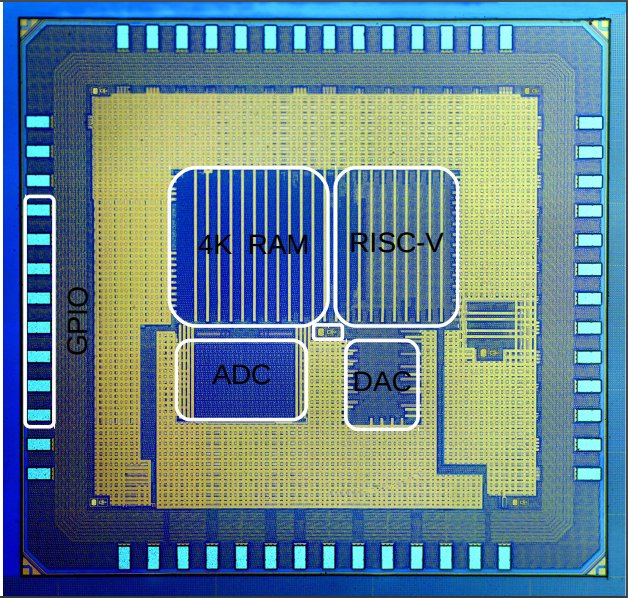
\includegraphics[width=0.5\textwidth]{figuras/riscv.jpg}
\end{figure}

\abreviatura{DAC}{\textit{Digital-to-Analog Converter}}
\abreviatura{RAM}{\textit{Random Access Memory}}
\abreviatura{RISCV}{\textit{Reduced Instruction Set Computing - V}}

Se nas ultimas décadas, o acesso a computadores se tornou facilitada, nas próximas que estão por vir, o uso e aquisição de sistemas computacionais não será um mero luxo ou aquisição, mas sim uma inevitabilidade. Tudo terá um processador, se não, um sistema computacional simples. Pode-se notar muitas etiquetas de RFID e cada vez mais modernas \cite{ricci2008design}, contendo sistemas computacionais complexos.

\subsection{Microprocessador}

Parte principal de um sistema computacional, com o objetivo de decodificar e executar as instruções em código de maquina existente na memória. A tabela que é interpretada, denominada por conjunto de instruções, contem todos os padrões binários possíveis a serem decodificados, resultando em sinais lógicos para a eletrônica que o executará, podendo realizar comparações, somas,multiplexações e leituras/escritas na memória.

Com o passar dos anos, o poder de processamento permitiu que sistemas simples possam ter grande valor intelectual agregado, podendo utilizar como exemplo o termostato da Google, vendido atualmente por \$250, por realizar um \textit{aprendizado de maquina}\footnote{"Campo de estudo que dá aos computadores a habilidade de aprender sem serem explicitamente programados`` -  Arthur Samuel, 1945.}, proporcionando ao aparelho um melhor gerenciamento da temperatura do ambiente, realizando uma economia energética e uma melhora na qualidade de vida do usuário.

\subsection{SoC}

Atualmente o termo é empregado a circuitos integrados com uma vasta quantidade de sistemas integrados, podendo citar  \textit{GPU} (\textit{Graphics Processing Unit}), \textit{USB} (\textit{Universal Serial Bus}), módulos de rede, rádio e outros sistemas dentro do próprio circuito integrado.

\abreviatura{GPU}{\textit{Graphics Processing Unit}}
\abreviatura{USB}{\textit{Universal Serial Bus}}

Nesta categoria, pode-se destacar o desenvolvimento dos sistemas desenvolvidos pela fabricante ARM, tendo ultrapassado a Intel como a maior produtora de processamentos do mundo, após a revolução \textit{mobile} onde a maioria das pessoas comuns começaram a utilizar \textit{smartphones} substituindo o uso de computadores pessoais para realizar as suas rotinas pessoais digitais diárias. Esta revolução, esta fazendo uma grande modificação no ambiente de desenvolvimento das grandes empresas, permitindo o desenvolvimento de hardware sem a necessidade de empresas altamente especializadas para desenvolvimento, tornando um foco de desenvolvimento genérico e macroscópico.


\section{Bootloader}

A vantagem de se utilizar um sistema de carregamento de boot\footnote{Processo no qual o sistema computacional se inicia.} é
a gravação programa principal com a assistência de um software primário, conhecido como \textit{bootloader}. Um microcontrolador
com este sistema, também pode ser denominado de auto-programável, pois possui as dependências necessárias para realizar o próprio
processo de programação.

Contudo, é importante a realização da programação externa, utilizando um \textit{hardware} especializado, que permiti a programação do processador, independente do \textit{software} que já está programado ou em execução. Alguns processadores, que se encontram em estados indevidos ou não planejados, podendo acarretar um mal funcionamento do sistema, podem ser regravados sem a preocupação do \textit{bootloader}, utilizando a gravação com a ferramenta do \textit{hardware} especializado, limpando toda a memória e gravando o programa. O mesmo também é necessario para realizar a gravação do bootloader pela primeira vez no processador, após isso, o próprio bootloader pode se reprogramar ou atualizar.

Para entender melhor o funcionamento, pode-se utilizar uma maquina de estados do \textit{bootloader} utilizado nos microcontroladores
AVR, para uma melhor visualização na \figref{fig:sm_bootloader} e uma descrição dos estados na \tabref{tab:bootloader}.

\begin{figure*}[ht!]
  \centering
  \begin{tikzpicture}[->,>=stealth',shorten >=1pt,auto,node distance=2.8cm,
                      semithick]
    \tikzstyle{every state}=[fill=blue,draw=none,text=white]

    \node[inicio,state]  (A)                    {$init\_hw$};
    \node[state]         (B) [right of=A]       {$new\_prg$};
    \node[state]         (C) [below of=B]       {$get\_com$};
    \node[state]         (D) [left of=C]        {$chk\_com$};
    \node[state]         (E) [left of=D]        {$exe\_com$};
    \node[state]         (F) [right of=B]       {$run\_prg$};

    \path (A) edge              node {}      (B)
          (B) edge              node {sim}   (C)
              edge              node {não}   (F)
          (C) edge              node {}      (D)
          (D) edge              node {correto}      (E)
              edge [bend right] node [above] {erro} (C)
          (E) edge [bend right] node [below] {}     (C);
  \end{tikzpicture}
  \caption[Máquina de estados do avr \textit{bootloader}]{\label{fig:sm_bootloader}}{Máquina de estados
  do avr \textit{bootloader},\\ baseado em \textit{AVR109: Self Programming - ATMEL}.}
\end{figure*}

\begin{table}[ht!]
\centering
\caption[Descrição dos estados do bootloader]{Descrição dos estados da \figref{fig:sm_bootloader}}
\label{tab:bootloader}
\begin{tabular}{@{}l l p{55mm}@{}}
\toprule
Estado             & Próximos estados           & Descrição                                                                                                             \\ \midrule
\textit{init\_hw}  & \textit{new\_prog}         & Inicializa depêndencias de \textit{hardware} para a utilização do \textit{bootloader}, Ex: serial.                \\
\textit{new\_prog} & \textit{get\_com,run\_prg} & Espera uma interrupção de \textit{hardware} ser inicializada para inicialização da rotina de \textit{bootloader}. \\
get\_com           & \textit{chk\_com}          & Adiquiri os dados do \textit{buffer} da serial.                                                                     \\
chk\_com           & \textit{exe\_com,get\_com} & Checa o comando recebido pela serial, caso o não é valido outro comando deverá ser buscado.                           \\
exe\_com           & \textit{get\_com}          & Executa o comando após a validação                                                                                    \\
run\_prg           &                            & Inicializa programa principal caso a rotina de programação não é inicializada via interrupção de \textit{hardware}. \\ \bottomrule
\end{tabular}
\end{table}

O \textit{bootloader}, por ser uma peça de software essencial dos sistemas auto-programáveis, ele se encontra na parte da memória
não volátil, existindo dentro de uma faixa determinada da memória ao lado do programa principal que será executado, como pode ser
visualizado na \figref{fig:me_bootloader}.

\begin{figure*}[ht!]
  \centering
  \begin{bytefield}{24}
    \memsection{ffff ffff}{002f c000}{15}{Pilha}\\
    \begin{rightwordgroup}{Flash}
        \memsection{002f bfff}{0001 0000}{9}{Aplicação principal}\\
        \memsection{0000 ffff}{0000 0000}{3}{\textit{Bootloader}}
    \end{rightwordgroup}\\
  \end{bytefield}
  \caption[Memória com \textit{bootloader}]{\label{fig:me_bootloader}}{Memória com bootloader,\\baseado em
  \textit{``Modular bootloader framework for silicon labs SIMXXXXX microcontrollers - Silicon Labs''}.}
\end{figure*}

%\subsection{Gravação}
%O processo é a transmissão do novo código a ser enviado para a memória do sistema embarcado, r

%\itodo{[ADICIONAR  UMA LISTA DOS BOOTLOADERS]}
\section{KDevelop}
O plugin proposto foi desenvolvido encima da plataforma conhecida como \textbf{KDevelop}, pertencente a organização \textit{KDE},
sendo um conceito de \textit{IDE} para programação.

Concebido utilizando as tecnologias de código aberto mais modernas, como C++14, QT 5.8, entre outras bibliotecas e ferramentas
utilizadas, podendo assim denominar o sistema como \textit{Rolling release}\footnote{Sistemas de software que atualizam suas bases
de código para a utilização das ultimas versões das ferramentas empregadas no projeto.}.

O \textbf{KDevelop} teve seu primeiro lançamento em 1999, sendo majoritariamente programado em C++, podendo ser utilizado
para programar em C, C++, Perl, Python, PHP, Java, Fortran, Ruby, Ada, Pascal, SQL e Bash. Suportando também sistemas de
configuração para compilação como: cmake, qmake e make.

Diferente de outras \textit{IDEs} que propõem as mesmas soluções que o \textbf{KDevelop}, este é inteiramente desenvolvido
com foco em performance e numa agradável experiência do usuário, permitindo o desenvolvimento e adesão de projetos na \textit{IDE},
sem a burocracia da adesão do projeto na interface, permitindo utilizar toda a informação disponível nos sistemas assistencialistas
de configuração de compilação, como fonte das dependências e de informações sobre o projeto adicionado. Para um programador comum
de código aberto, \textbf{KDevelop} se apresenta como uma ótima opção.

\abreviatura{IDE}{\textit{Integrated Development Environment}}

\subsection{Google Summer of Code}
O projeto foi financiado pela \textbf{Google}, como parte do \textit{Google Summer of Code} (\figref{fig:gsoc2016}) durante
sua realização, como incentivo de desenvolvimento pra organizações e projetos de código aberto. A proposta do desenvolvimento
de um plugin para sistemas embarcados na \textit{IDE} \textbf{KDevelop}, foi submetida e aprovada pela organização
responsável (\textit{KDE}).

\begin{figure}[!htb]
  \centering
  \caption[Logo GSoC 2016]{Logo do projeto \textit{Google Summer of Code} 2016}
  \label{fig:gsoc2016}
  
\includegraphics[width=0.7\textwidth]{figuras/gsoc2016.jpg}
\end{figure}

\subsection{Plugins}
O \textit{plugin} opera como uma biblioteca compartilhada que é carregada durante o tempo de execução, desta forma, providenciando acesso
as funções da biblioteca. A vantagem de se lhe utilizar, é a instalação dos \textit{plugins} que são utilizados, permitindo desta forma
um uso modular das dependências utilizadas no projeto, sem a necessidade de ter o conjunto como um único binário com todas as dependências,
mesmo aquelas não utilizadas pelo desenvolvedor.

Uma outra vantagem da utilização de \textit{plugins}, é permitir somente a utilização do binário, sem a necessidade de utilizar
o código fonte do mesmo, permitindo desta forma, a utilização de \textit{plugins} que não são de código aberto, facilitando desta
forma o apoio e uso de sistemas proprietários desenvolvidos, mantendo sigiloso o trabalho intelectual do mesmo.

\subsection{Comunidade Open Source}

A comunidade pertencente a cultura \textit{Open Source}\footnote{Projetos desenvolvidos de código aberto, podendo ser utilizado,
modificado e reproduzido.}, tem como base o usufruto dos trabalhos produzidos, pela mesma, para a humanidade \cite{wynants2005open},
permitindo a copia, distribuição, estudo, alteração e melhoraria do software \cite{filosofia},
tornando o código altamente configurável, flexível e facilmente atualizável para suportar as versões mais novas
de suas dependências.

% http://pt.slideshare.net/ezyolamarca/palestra-ezyo-usodeferramentaslivresnagestaodoconhecimentoodp
A base desta cultura é a \textit{CoP}\footnote{Denominação dada a um grupo de indivíduos que tem um interesse comum,
compartilhando o desenvolvimento e conhecimento para uma finalidade comum.}\cite{wenger1998communities}, tendo como foco o desenvolvimento,
paralelo e continuo de produtos de código aberto para uma finalidade especial que o grupo propõem, em pró a civilização. Permitindo
que qualquer um possa ter direito completo ao acesso e apropriação do material intelectual concebido pela comunidade.

\abreviatura{CoP}{\textit{Communities of Practice}}

O termo, mesmo sendo utilizado majoritariamente para software, também é empregado para produtos de hardware desenvolvidos,
podendo também ser denominado como \textit{Open Hardware} (\figref{fig:osoh}).

\begin{figure}[!htb]
  \centering
  \caption[\textit{Open Software} e \textit{Open Hardware} logos]{Logos utilizadas em projeto de software na esquerda e de hardware à direita.}
  \label{fig:osoh}
  
\includegraphics[width=1\textwidth]{figuras/osoh.png}
\end{figure}

Durante os últimos anos, com a evolução tecnológica da informação, permitindo que as pessoas tenham um acesso mais aberto para
a tecnologia, permitiu que a evolução das comunidades de código aberto, e o numero de pessoas que fazem parte destas, tivessem
um crescimento exponencial de membros, resultando em projetos extremamente populares e de um valor intelectual incalculável,
pela vasta quantidade e especializações necessárias para sua concepção. Entre os projetos mais populares de software e hardware
abertos, podem se destacar a kernel do sistema operacional conhecido como \textbf{Linux} e os projetos de impressoras 3D, tendo
como destaque a \textbf{RepRap}.

\subsection{KDE}
Existe uma grande quantidade de organizações de código aberto, estre elas, pode-se destacar: \textit{Linux Foundation}, KDE, GNOME,
GNU entre inúmeras outras. O trabalho aqui relatado foi desenvolvido para a organização KDE, que tem como lema principal: ``Experimente
a liberdade'' \cite{kdelema}, deixando de forma implícita os teóricos malefícios de produtos com código fechado\footnote{Denominado pela
comunidade como \textit{Software Closed Source}}.

A comunidade teve seu inicio em 1996 como uma tentativa de ambiente de trabalho para computadores, com o objetivo
de tornar a experiência do usuário simples e agradável, tanto a interface de usuário como os programas utilizados no computador.
No Brasil, existe aproximadamente 50 milhões de estudantes usando sistemas baseados nas tecnologias desenvolvidas pela KDE
\cite{kdewhatis}.

\section{Sistema de Controle de Versão}

Para fazer o controle do projeto desenvolvido, dentre as ferramentas utilizadas, foi realizado todo o desenvolvimento com o
\textit{GIT} (\figref{fig:gitlogo}), sendo uma das opções mais comuns entre as comunidades da cultura \textit{Open Source}
ao lado do sistema conhecido como bazaar.

\abreviatura{GIT}{\textit{Global Information Tracker}}

\begin{figure}[!htb]
  \centering
  \caption[Logo GIT]{Logo do sistema de controle de versão GIT.}
  \label{fig:gitlogo}
  
\includegraphics[width=0.4\textwidth]{figuras/gitlogo.png}
\end{figure}

A maior utilidade de um sistema que permiti o controle de versão de código, é permitir a realização do trabalho em paralelo,
detecção de conflitos entre diferentes versões, rastrear modificações, detecção de erros, entre outras utilizações de grande valia
para o desenvolvimento de software.
